\subsection{Apache Spark}
\label{sec:spark}
Apache Spark è un framework per la computazione di grandi moli di dati
su cluster, progettato e implementato nel 2010 da un gruppo di ricercatori dell’Università di Berkeley a San Francisco \cite{spark:hadoop}. Viene scherzosamente descritto come "quello più veloce di Hadoop" perché nel confronto con il suo predecessore ha prestazioni 10-100 volte maggiori.
\\Questo progetto nasce dall'esigenza di migliorare le prestazioni dei sistemi distribuiti “MapReduce”. Ad alto livello infatti, un'applicazione Spark è formata da un driver program, che contiene la funzione main scritta dall'utente, e di una serie di parallel operation definite nel programma che verranno eseguite sui vari nodi worker che compongono il cluster. Fin qui nulla di nuovo, è il modello del calcolo distribuito master/slave. La vera innovazione è stata introdotta nel modo di definire i dati da elaborare.
\\Infatti Spark mette a disposizione un'astrazione molto potente, il \textit{resilient distribuited dataset} (RDD), che rappresenta una collezione di dati "immutabili" a cui il programmatore si può riferire direttamente tramite l'oggetto associato. Un RDD rappresenta un set di dati che è suddiviso in partizioni (Una tabella chiave-valore suddivisa in tante sotto-tabelle o un file diviso in tanti segmenti). 
\\L’RDD realizza la fault tolerance grazie all'informazione di lineage: quando una partizione di un RDD si perde a causa di un guasto o di un altro errore, l’RDD ha tutte le informazioni riguardo la storia di quella partizione, in termini di operazioni effettuate su di esso che gli consentono di ricostruirla. La creazione, avviene a partire dai dati su disco (presi da HDFS) o da altre fonti di dati. Una volta creato, un RDD può restare in memoria centrale oppure può essere materializzato su disco.
\begin{figure}[H]
	\centering
	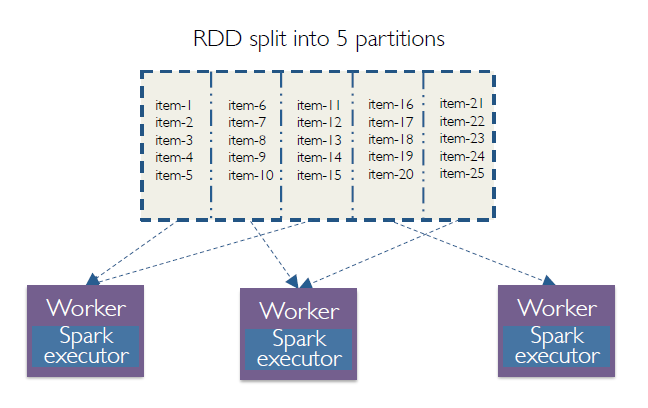
\includegraphics[width=\textwidth]{images/sparkRDD.png}
	\caption{Visualizzazione di un RDD partizionato.}
	\label{fig:sparkRDD}
\end{figure}
Spark nasce come un sistema per creare e gestire job di analisi basati su trasformazioni di RDD. Dato che gli RDD nascono e vivono in memoria, l’esecuzione di lavori iterativi, o che trasformano più volte un set di dati, sono immensamente più rapide di una sequenza di MapReduce; questo perchè il disco non viene mai (o quasi mai) impiegato nell'elaborazione.
\\Il vantaggio principale dell'utilizzo di Spark è la sua estrema velocità nell’eseguire programmi di elaborazione dati. Il motivo di queste prestazioni risiedono in una miglior gestione della memoria; aspetto che lo diversifica da Hadoop. Prendendo come esempio una generica elaborazione fatta con il paradigma MapReduce, in Hadoop questa produce il seguente schema di lavoro, che può essere iterato più volte (semplificando):
\begin{itemize}
\item Load dei dati da disco locale verso i nodi worker del cluster;
\item Esecuzione della funzione assegnata;
\item Store dei dati su disco locale.
\end{itemize}
Le ripetute fasi di load/store rendono il sistema complessivamente lento. Spark, invece, cerca di mantenere in memoria i dati, esegue le operazioni di trasformazione e solo alla fine memorizzare i dati sul disco.
\\Come detto in precedenza, Spark non utilizza MapReduce come motore di esecuzione; invece, utilizza il proprio runtime distribuito (DAG) per l’esecuzione di jobs su un cluster. Quando viene invocata un’azione su un RDD, viene creato un “job”. Un Directed Acyclic Graph o DAG è un grafo aciclico in cui ogni nodo è una partizione di RDD e ogni vertice è una trasformazione. A differenza di MapReduce, il motore DAG di Spark può processare pipeline arbitrarie di operatori e tradurle in un unico “job” per l'utente.
\\Spark, infine, sta dimostrando di essere una buona piattaforma su cui costruire strumenti di analisi, infatti ha moduli per il Machine learning (MLlib), Elaborazione grafica (GraphX), Elaborazione di stream (Spark Streaming) ed SQL (Spark SQL) \cite{spark:hadoop}.
\begin{figure}[H]
	\centering
	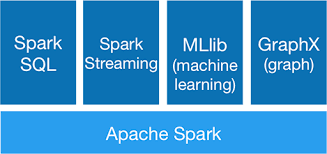
\includegraphics[width=\textwidth]{images/spark.png}
	\caption{Infrastruttura Spark.}
	\label{fig:sparkOverview}
\end{figure}
\subsubsection{Spark Streaming}
\label{sub:spark streaming}
Nel sistema distribuito, poichè c'è l'esigenza di recuperare i dati in real time dalla coda di bitcoind, viene utilizzato Spark Streaming. Questo modulo è un'estensione dell'API Spark di base che consente l'elaborazione streaming, scalabile, ad alto throughput e con tolleranza agli errori dei flussi di dati in tempo reale. I dati, che possono provenire da diverse fonti, sono elaborati utilizzando algoritmi complessi espressi con funzioni di alto livello come \textit{map}, \textit{reduce}, \textit{join} e \textit{window}. I dati processati, infine possono essere inviati a filesystem (Hadoop) o database (Neo4j) per il salvataggio oppure ad altri moduli di Spark, dediti all'analisi, tipo machine learning (MLlib) o graph processing (GraphX). 
\\Internamente, Spark Streaming riceve streams di dati di input e li divide in batch, che vengono quindi elaborati dal motore Spark per generare il flusso finale di risultati. Per consentire il facile utilizzo di questi dati, fornisce un'astrazione di alto livello chiamata stream discretizzato o DStream, che rappresenta un flusso continuo di dati. E' possibile creare Dstreams da flussi di dati di input da sorgenti come Kafka, Flume e Kinesis o applicando operazioni di alto livello su altri Dstreams \cite{spark:home-streaming}. Internamente, un Dstream è rappresentato come una sequenza di RDD sulla quale possono essere effettuate le operazioni descritte in precedenza. Infatti, i Dstream possono essere trasformati usando le operazioni di trasformazione simili a quelle dei RDD, come map e filter.
\begin{figure}[H]
	\centering
	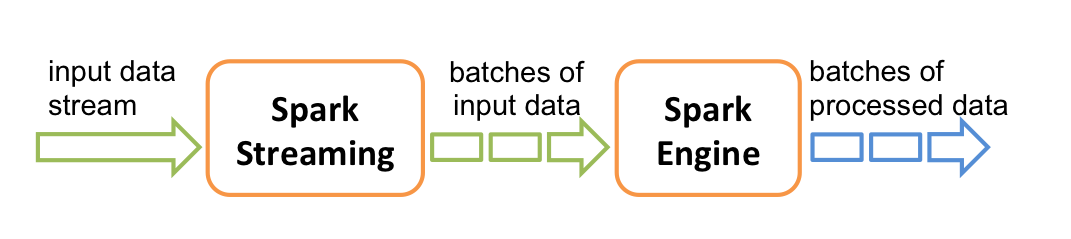
\includegraphics[width=\textwidth]{images/streamingSpark.png}
	\caption{Come vengono gestiti i dati in Spark Streaming.}
	\label{fig:streamingSpark}
\end{figure}
\subsubsection{GraphX}
\label{sub:graphX}
La diffusione dei grafi nei sistemi informatici ha portato a un grande lavoro di analisi su di essi. Facendone un utilizzo sempre più frequente, ci si trova a dover fare ricerche, interrogazioni e misure su questa struttura dati e di trovare un modo per memorizzare efficientemente questi oggetti. Anche Spark si è occupato del problema e ha reso disponibile uno strumento, basato sul framework principale, che ottimizza la gestione dei grafi e consente di applicare ad essi funzioni e metodi in modo molto intuitivo. Si tratta del progetto GraphX. Questo modulo è usato nel sistema distribuito, per fare analisi dei dati provenienti dall'elaborazione di Spark.
\\GraphX è un nuovo componetene di Apache Spark per grafi ed il calcolo parallelo su di essi.  Spark ha introdotto l'RDD, un'astrazione comoda per memorizzare i dati e risparmiando al programmatore parecchio lavoro. GraphX estende il concetto di RDD introducendo il \textit{Resilient Distribuited Graph} (RDG). Inoltre, per aiutare nell'analisi, espone un insieme di operatori fondamentali (sottografo, joinVertices e aggregateMessages) come variante ottimizzata dell'API Pregel. In più, Graphx include una crescente collezione di algoritmi e costrutti per grafi per semplificare le attività di analisi \cite{spark:graphx}. Attualmente le sue API sono scritte in Scala, Java e Python.
\begin{figure}[H]
	\centering
	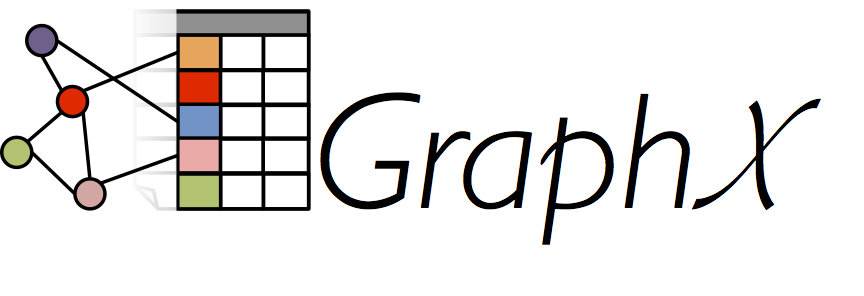
\includegraphics[width=\textwidth, height=0.15\textheight, keepaspectratio]{images/graphxLogo.png}
	\caption{Logo GraphX.}
	\label{fig:graphxLogo}
\end{figure}
GraphX, come detto in precedenza, gestisce i dati in memoria come se fossero grafi. Infatti, utilizza archi e vertici che hanno delle proprietà. Ogni vertice possiede un identificativo univoco a 64bit (VertexID), mentre, allo stesso modo, gli archi contengono gli identificativi di origine e partenza. Queste proprietà sono definite dal programmatore e tenuti in memoria come oggetti. Su di essi si possono eseguire metodi per l'analisi già inclusi nella libreria di GraphX come Connected components, Triangle Counting, PageRank, etc. Nell'elaborato di tesi, per trovare i nodi con maggior importanza all'interno del grafo, è stato usato l'algoritmo \textit{PageRank}.
\\Il PageRank è un algoritmo di analisi che assegna un peso numerico ad ogni elemento di un collegamento ipertestuale di un insieme di documenti, come ad esempio il World Wide Web, con lo scopo di quantificare la sua importanza relativa all'interno della serie. L'algoritmo di PageRank è stato brevettato (brevetto US 6285999) dalla Stanford University; è inoltre un termine ormai entrato di fatto nel lessico dei fruitori dei servizi offerti dai motori di ricerca. Il nome PageRank è un marchio di Google ed il suo nome si deve a Larry Page \cite{pageRank:google}, uno dei due fondatori di quell'azienda \cite{wiki:pageRank}.
\\L'algoritmo completo per il calcolo del PageRank fa ricorso all'uso della teoria dei processi Markov ed è classificato nella vera categoria degli algoritmi di Link Analysis Ranking. Dalla formula inizialmente sviluppata dai fondatori di Google, Sergey Brin e Larry Page, è possibile comprendere come il PageRank viene distribuito tra le pagine:
$$
PR[A] = \frac{1-d}{N} + d  (\sum_{K=1}^n \frac{PR[Pk]}{C[Pk]})
$$
Dove:
\begin{itemize}
\item \textbf{PR[A]} è il valore di PageRank della pagina A che vogliamo calcolare.
\item \textbf{N} è il numero totale di pagine note.
\item \textbf{n} è il numero di pagine che contengono almeno un link verso A. Pk rappresenta ognuna di tali pagine.
\item \textbf{PR[Pk]} sono i valori di PageRank di ogni pagina Pk.
\item \textbf{C[Pk]} sono il numero complessivo di link contenuti nella pagina che offre il link.
\item \textbf{d (damping factor)} è un fattore deciso da Google e che nella documentazione originale assume valore 0,85. Può essere aggiustato da Google per decidere la percentuale di PageRank che deve transitare da una pagina all'altra e il valore di PageRank minimo attribuito ad ogni pagina in archivio.
\end{itemize}
Dalla formula si nota quindi che all'aumentare del numero di link complessivi dei siti che puntano ad A il PageRank aumenta.

\subsection{Hadoop HDFS}
\label{sec:hadoop HDFS}
Apache Hadoop è un framework open-source che supporta applicazioni distribuite con elevato accesso ai dati, è uno dei primi sistemi per l’analisi di Big Data, ed è stato considerato un modello da seguire per tutti i sistemi che sono stati creati successivamente. Apache Hadoop è stato ideato per la memorizzazione e la gestione di grandi quantità di dati in parallelo, su cluster di grandi dimensioni (costituiti da migliaia di nodi) assicurando un'elevata affidabilità, scalabilità e disponibilità (fault-tolerant). Tutti i moduli, infatti, sono progettati in modo tale che il software del framework gestisca automaticamente gli eventuali “down” dell’hardware, molto frequenti in un sistema parallelo.
\\Hadoop nacque per sopperire a un grave problema di scalabilità di Nutch, un crawler open source basato sulla piattaforma Lucene di Apache. I programmatori Doug Cutting e Michael J. Cafarella hanno lavorato a una versione iniziale di Hadoop a partire dal 2004; proprio in quell’anno furono pubblicati documenti tecnici riguardanti il Google File System e Google MapReduce, documenti da cui Doug e Michael attinsero le competenze fondamentali per lo sviluppo di HDFS e di un nuovo e innovativo pattern per l’elaborazione distribuita di elevate moli di dati, MapReduce, che oggi rappresenta uno dei componenti fondamentali di Hadoop. Circa quattro anni più tardi, nel 2008, nacque la prima release come progetto Open Source indipendente di Apache. A oggi Hadoop è un insieme di progetti tutti facenti parte della stessa infrastruttura di calcolo distribuito.
\\Hadoop offre librerie che permettono la suddivisione dei dati da elaborare direttamente sui nodi di calcolo e permette di ridurre al minimo i tempi di accesso, questo perché i dati sono immediatamente disponibili alle procedure senza pesanti trasferimenti in rete. Il framework garantisce inoltre un’elevata affidabilità: le anomalie e tutti gli eventuali problemi del sistema sono gestiti a livello applicativo anziché utilizzare sistemi hardware per garantire alta disponibilità. Un’altra caratteristica di Hadoop è la scalabilità che è realizzabile semplicemente aggiungendo nodi al cluster in esercizio. I principali vantaggi di Hadoop risiedono nelle sue caratteristiche di agilità e di flessibilità.L’architettura base del framework Hadoop, si compone dei seguenti elementi principali:
\begin{itemize}
\item  \textbf{HDFS}: Il filesystem distribuito di Hadoop, nella quale vengono fisicamente salvati i file.
\item  \textbf{MapReduce}: Un framework per la creazione di applicazioni in grado di elaborare grandi quantità di dati in parallelo basandosi sul concetto di functional programming, ed è, quindi, il principale responsabile del processo di calcolo.
\item  \textbf{Yarn}: Si occupa della schedulazione dei task, ossia delle sotto-attività che compongono le procedure map e reduce eseguite nel processo di calcolo.
\end{itemize}
\begin{figure}[H]
	\centering
	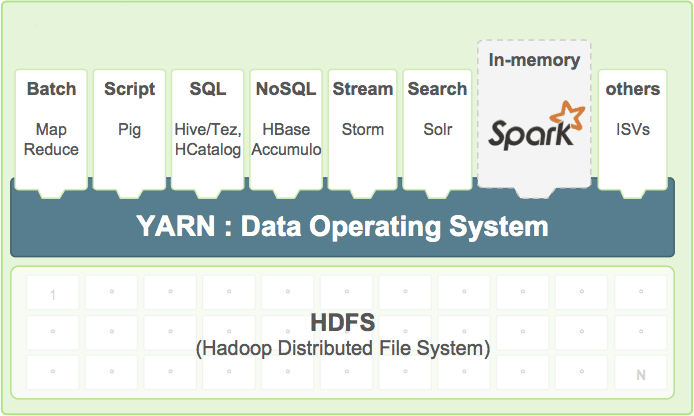
\includegraphics[width=\textwidth, height=0.30\textheight, keepaspectratio]{images/HDFSSpark.png}
	\caption{Visualizzazione invio dati ad HDFS.}
	\label{fig:HadoopHDFS}
\end{figure}
All'interno del sistema distribuito, per il salvataggio veloce e distribuito dei dati su dispositivi fisici, viene utilizzato l'HDFS di Hadoop.
\\L'HDFS (Hadoop Distributed File System), come riportato nella documentazione ufficiale, è il file system distribuito di Hadoop, progettato appositamente per immagazzinare un'enorme quantità di dati (dell'ordine dei Gigabyte e Terabyte), in modo da ottimizzare le operazioni di archiviazione e accesso a un ristretto numero di file di grandi dimensioni, a differenza dei tradizionali file system che sono ottimizzati per gestire numerosi file di piccole dimensioni; infatti, quando la mole dei dati diventa non più gestibile da una singola macchina, si rende necessario partizionare gli stessi su un certo numero di macchine separate, interconnesse da una rete (cluster), rendendo il filesystem di fatto distribuito. 
\\HDFS presenta i file organizzati in una struttura gerarchica di cartelle. Dal punto di vista dell'architettura, un cluster è costituito dai seguenti tipi di nodi: 
\begin{itemize}
\item  \textbf{NameNode}: è l'applicazione che gira sul server principale. Gestisce il file system e in particolare il namespace, Inoltre, determina come i blocchi dati siano distribuiti sui nodi del cluster e la strategia di replicazione che garantisce l’affidabilità del sistema. Il NameNode monitora anche che i singoli nodi siano in esecuzione senza problemi e in caso contrario decide come riallocare i blocchi. 
\item  \textbf{DataNode}: applicazione/i che girano su altri nodi del cluster, generalmente una per nodo, e gestiscono fisicamente lo storage di ciascun nodo. Queste applicazioni eseguono, logicamente, le operazioni di lettura e scrittura richieste dai client e gestiscono fisicamente la creazione, la cancellazione o la replica dei blocchi dati. 
\item  \textbf{SecondaryNameNode}: si tratta di un servizio che aiuta il NameNode a essere più efficiente 
\item  \textbf{BackupNode:} è il nodo di failover e consente di avere un nodo simile al SecondaryNameNode sempre sincronizzato con il NameNode.
\end{itemize}
In HDFS le richieste di lettura dati seguono una politica relativamente semplice \cite{hadoop:HDFS} avvengono scegliendo i nodi più vicini al client che effettua la lettura e, ovviamente, in presenza di dati ridondati, risulta più semplice soddisfare questo requisito. Inoltre, occorre precisare che la creazione di un file non avviene direttamente attraverso il NameNode. Infatti, il client HDFS crea un file temporaneo in locale e solo quando tale file supera la dimensione di un blocco, è preso in carico dal NameNode. Quest’ultimo crea il file all’interno della gerarchia del file system, identifica un DataNode e i blocchi su cui posizionare i dati. Successivamente DataNode e blocchi sono comunicati al client HDFS che provvede a copiare i dati dalla cache locale alla sua destinazione finale.
\begin{figure}[H]
	\centering
	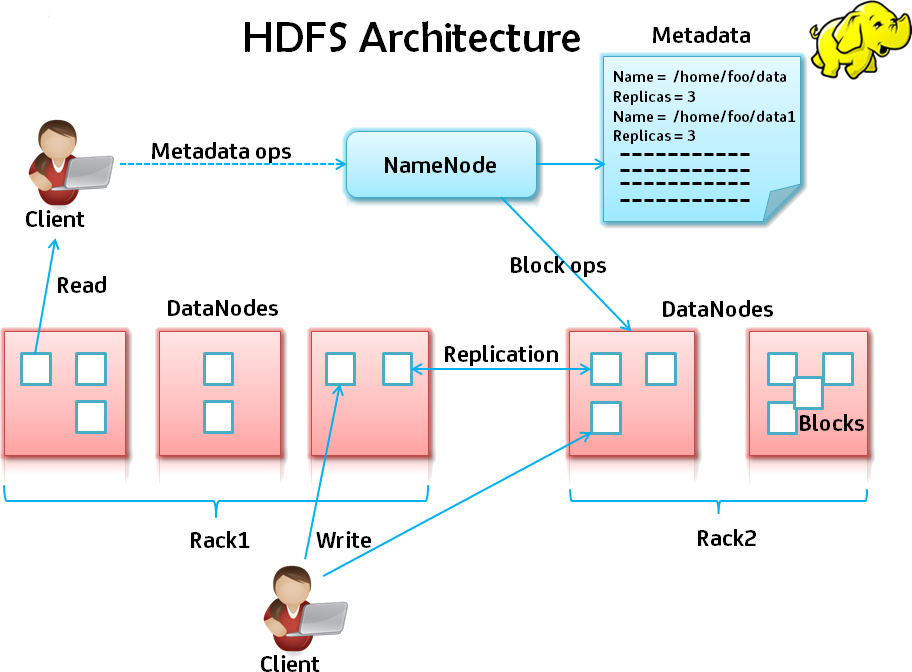
\includegraphics[width=\textwidth, height=0.40\textheight, keepaspectratio]{images/HDFSArchitetture.png}
	\caption{Architettura HDFS.}
	\label{fig:HadoopHDFS}
\end{figure} 
Quanto detto fino a ora, ci permette di concludere che quando vengono trattati file di grandi dimensioni, HDFS è molto efficiente. Invece con file di piccole dimensioni, dove per piccole dimensioni s'intendono dimensioni inferiori al blocco, il trattamento dei file è molto inefficiente, questo perché i file utilizzano spazio all'interno del namespace, cioè l'elenco dei file mantenuti dal NameNode, che ha un limite dato dalla memoria del server che ospita il NameNode stesso. 

\subsection{Neo4j}
\label{sec:neo4j}
Negli ultimi anni è incredibilmente aumentata la popolarità delle tecnologie di immagazzinamento di informazioni conosciute con il nome di \textit{NoSQL}, acronimo che sta per Not only SQL \cite{neo4j:NoSQL}. I NoSQL \textit{Database Management System (DBMS)} sono sistemi software che consentono di immagazzinare e organizzare i dati senza fare affidamento sul modello relazionale, solitamente impiegato da database tradizionali.
\\I NoSQL DBMS sono inoltre contraddistinti dal fatto che non utilizzano un sistema transazionale ACID e spesso sono schema-less \cite{neo4j:NoSQL}, ovvero non possiedono uno schema fisso a cui devono attenersi, evitando spesso così le operazioni di join.
\\Le strutture dei dati memorizzati nei sistemi NoSQL (ad esempio documenti, grafi o coppie chiave/valore) rendono alcune operazioni più veloci rispetto a generici database relazionali. Si utilizzano infatti diversi tipi di database NoSQL in base al problema da risolvere. Le tipologie di database NoSQL più utilizzate sono:
\begin{itemize}
\item  \textbf{Key/Value Store}: rappresentano una tipologia di database NoSql che si basa sul concetto di \textit{associative array}, implementati attraverso HashMap. In un array associativo si hanno un insieme di record che possono essere identificati sulla base di una chiave univoca. La tipologia di memorizzazione adottata dai key/value stores garantisce tempi di esecuzione costanti per tutte le operazioni applicabili sui dati: \textit{add, remove, modify e find}.
\item  \textbf{Document-oriented database}: questo tipo di database permette di memorizzare in maniera efficiente dati semistrutturati. Essi possono essere considerati una specializzazione dei database key/value, nei quali vengono permesse strutture innestate. Sono spesso usati i formati JSON o XML per la memorizzazione dei dati. MongoDB è il più diffuso database orientato ai documenti ed è uno dei DBMS NoSQL più utilizzati.
\item  \textbf{Column-oriented database}: i DBMS colonnari, a differenza dei tradizionali RDBMS, che memorizzano i dati riga per riga, sfruttano la memorizzazione dei dati per colonna. Per ogni colonna si memorizzano coppie chiave/valore, dove la chiave è l'identificativo di riga ed il valore è il valore associato a quella colonna per la specifica riga. Questa rappresentazione permette di risparmiare una notevole quantità di spazio in caso di sparsità dei dati.
I DBMS di tipo colonnare più diffusi sono HBase e Cassandra.
\item  \textbf{Graph database}: un database a grafo utilizza un insieme di nodi con un insieme di archi che li connettono per memorizzare le informazioni, in cui le “relazioni” vengono rappresentare come grafi. Le strutture a grafo si prestano molto bene per la rappresentazione di determinati dati semistrutturati e altamente interconnessi come, ad esempio, i dati dei social network e del Web. I database a grafi più diffusi sono GraphDB, OrientDB e Neo4j.
\end{itemize}
La struttura dati che più si avvicina all'idea di transazione è quella del grafo, con nodi che rappresentano i mittenti/destinatari dei bitcoin e gli archi che identificano l'ammontare della transazione. Per questo motivo, nel sistema distribuito, si è preferito fare utilizzo del database NoSQL Neo4j per il salvataggio. Inoltre, le performance dei Graph DBMS tendono ad essere ottimali quando i dati da archiviare sono altamente connessi e la mole del dataset è estremamente grande. Questo perché al contrario degli RDBMS (Relational Database Management System), la loro natura gli consente di evitare le onerose operazioni di join semplicemente attraversando le relazioni che connettono i nodi.
\\Neo4j, dunque, è un software per basi di dati a grafo open source sviluppato interamente in Java. È un database totalmente transazionale, che viene integrato nelle applicazioni permettendone il funzionamento stand alone e memorizza tutti i dati in una cartella. È stato sviluppato dalla Neo Technology, una startup di Malmö, Svezia e della San Francisco Bay Area \cite{neo4j:wiki}. Il database può essere usato sia in modalità embedded che server. Nella modalità embedded si incorpora il database nell'applicazione (con maven o includendo i file JAR) e questo viene eseguito all'interno della JVM, quindi nello stesso processo ma accettando vari thread concorrenti. Nella modalità server invece il database è un processo a sé stante a cui si accede tramite REST facendo delle query e ricevendo i dati in remoto.
\\É robusto, scalabile e ad alte prestazioni. È dotato di:
\begin{itemize}
\item Transazioni ACID.
\item High Availability.
\item Può memorizzare miliardi di nodi e relazioni.
\item Alta velocità di interrogazione tramite attraversamenti.
\item Linguaggio di interrogazione dichiarativo e grafico chiamato Cypher
\item DBMS schema-less, ciò sta a significare che i suoi dati non devono attenersi al alcuna struttura di rifermento prefissata.
\end{itemize}
La index-free adjancency è alla base delle sue alte prestazioni di attraversamento, d'interrogazione e di scrittura, ed è uno degli aspetti chiave della sua architettura. L’index-free adjancency è una lista ( o tabella), ove ogni suo elemento è composto da un nodo del grafo e dai puntatori ai nodi connessi ad esso.
\\Neo4j, inoltre, salva i dati dentro di una serie di store file, contenuti all'interno di un'unica cartella. Ognuno di questi file contiene al suo interno le informazioni relative ad una singola parte del grafo (e.g. nodi, relazioni, proprietà). Questa separazione della struttura del grafo facilita il suo attraversamento. In Neo4j le unità fondamentali che compongono un grafo, dunque, sono i nodi e le relazioni. I nodi vengono solitamente impegnati per rappresentare le entità, ma a seconda della sfera delle relazioni possono essere utilizzati per scopi differenti. A parte proprietà e relazioni, i nodi possono anche essere etichettati con zero o più Label. Le relazioni tra i nodi, invece, sono una parte chiave dei database a grafo. Ci permettono di trovare le informazioni connesse. Come per i nodi, le relazioni possono avere le proprietà, hanno sempre una direzione e possiedono sempre un nodo di partenza e uno di arrivo. Infine, una label è un \textit{named graph construct} , viene usata per raggruppare i nodi in sottoinsiemi; tutti i nodi etichettati con la stessa label fanno parte dello stesso insieme.
\begin{figure}[H]
	\centering
	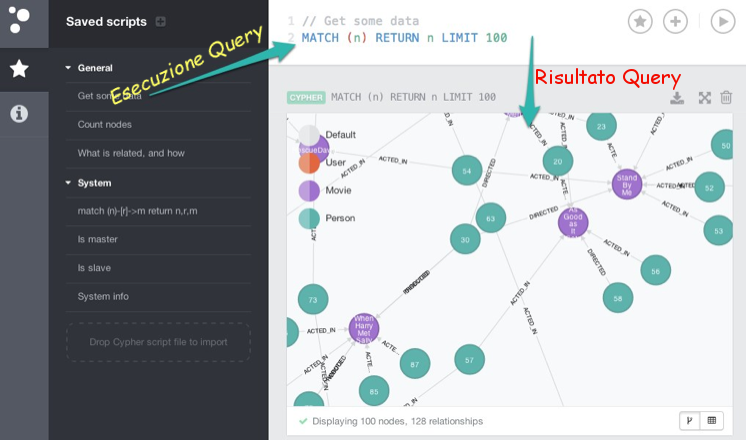
\includegraphics[width=\textwidth, height=0.35\textheight, keepaspectratio]{images/neo4jWebPage.png}
	\caption{Interfaccia web di Neo4j nella quale è eseguita una query.}
	\label{fig:Neo4jWebPage}
\end{figure}
Tra i vantaggi che possiamo ottenere nell'utilizzo di Neo4j troviamo:
\begin{itemize}
\item \textbf{Distribuito}: Qualora si voglia garantire che il proprio sistema sia in grado di fornire un servizio di erogazione dei dati continuo, senza failure point e in grado di bilanciare e gestire un'enorme mole di richieste, Neo4j High Available (HA) è la risposta a questa esigenza. Neo4j HA, infatti, è stato progettato per rendere semplici, le transazioni da una singola macchina ad un una macchina multipla, senza dover cambiare la tipologia delle istanze che andranno a comporre il cluster.
\item \textbf{REST API}: Il server è munito di una ricca REST API che permettono ai client di spedire richieste in formato JSON per mezzo del protocollo HTTP. Le risposte vengono restituite all'interno di documenti JSON arricchiti con Hypermedia Links che mettono in risalto ulteriori caratteristiche del dataset. Sono molteplici le funzionalità messe a disposizione dalla REST API, ma il suo più grande vantaggio è quello di potervi accendere per mezzo di una semplice applicazione browser, come Firefox, Chrome o Internet Explorer.
\item \textbf{Platform Independence}: Dato che le informazioni contenute nel server vengono accedute per mezzo di documenti JSON spediti attraverso l’HTTP, le applicazioni client possono essere costruite su qualsiasi tipo di piattaforma, basta possedere delle librerie client HTTP.
\item \textbf{Scaling Independence}: Quando Neo4j viene eseguito in modalità server possiamo aumentare o diminuire il numero di componenti del cluster indipendente dal tipo di applicazione.
\item \textbf{Per-request transactional}: Ogni richiesta da parte del client viene eseguita come una singola transazione, atomicamente separata dalle altre. Tuttavia, la REST API fornisce un supporto per l'esecuzione di operazioni in batch (ovvero l'esecuzione “accorpata” delle operazioni). 
\end{itemize}
Neo4j, infine utilizza un sistema di query dichiarativo e grafico che prende il nome di Cypher. Esso è un linguaggio grafico, ovvero si basa sulla riproduzione grafica del sotto-grafo che si vuole estrarre. Con le query è possibile creare, modificare, eliminate e interrogare i dati del database. Il sotto-grafo riprodotto nelle query viene chiamato pattern, e per produrlo non servono strumenti particolari , ma basta seguire delle semplici regole che permettono di disegnarlo impiegando i caratteri ASCII ( i caratteri presenti sulla tastiera).
\\Cypher permette, quindi, agli utenti ( o ad una applicazione che agisce per conto dell'utente) di interrogare il database cercando i dati che corrispondono ad una specifica struttura. In termini da profano, chiediamo al database di \textit{"cercare tutti quegli oggetti simili o che assomigliano"} ad un certo pattern.
\begin{lstlisting}[language=Cypher, label=lst:CypherQuery, caption={Query Cypher.}]
Match (a:NODE_LABEL)-[r:RELATION_LABEL]->(b:NODE_LABEL) 
RETURN a,b,r;
\end{lstlisting}
Questo è un esmpio di query scritta col linguaggio Cypher. Questo pattern descrive un path (percorso), che connette (a) a (b) ritornando sia i nodi che le relazioni che soddisfano la query.